\documentclass{article}
\usepackage{graphicx} % Required for inserting images
\usepackage[polish]{babel}
\usepackage[T1]{fontenc}
\usepackage{enumitem}
\usepackage{float}
\usepackage{hyperref}
\usepackage{amsmath}

\title{Analiza zależności cen wybranych samochodów osobowych od ich parametrów i danych technicznych}
\author{Michał Maksanty}
\date{Maj 2024}

\begin{document}

\maketitle
\tableofcontents

\newpage

\section{Wstęp}
Poniższa praca będzie zajmować się badaniem zależności cen wybranych modeli samochodów osobowych (Volkswagen Golf, BMW Seria 3, Opel Corsa - wybrane generacje) w zależności od:
\begin{itemize}[itemsep=0mm]
    \item pojemności silnika,
    \item roku produkcji,
    \item mocy,
    \item rodzaju paliwa,
    \item typu nadwozia,
    \item przebiegu,
    \item koloru,
    \item stanu,
    \item skrzyni biegów,
    \item pochodzenia.
\end{itemize}
Następnie zostaną utworzone modele regresji i na podstawie przyjętej w późniejszej części pracy metryki, zostanie wybrany najlepszy model.

Pomysł projektu zainspirowany jest faktem dostępności dużej ilości samochodów na rynku wtórnym. Z tej racji chciałem sprawdzić jakie zależności rzeczywiście mają zastosowanie w przypadku takich danych - od czego cena jest bardziej zależna, a od czego mniej - taka analiza może ułatwić ewentualne poszukiwania samochodu i potencjalnie zwiększyć szansę na znalezienie auta w niższej cenie. A jej ciekawym efektem będzie oczywiście wybrany model najlepiej opisujący analizowane dane.

\section{Zbiór danych}
\subsection{Źródła danych}
Wstępne założenia projektu zakładały wykorzystanie jako źródła danych o samochodach platform internetowych: \href{https://www.olx.pl/}{OLX} oraz \href{https://www.otomoto.pl/}{OTOMOTO}.

\subsection{Pobieranie danych}
Dane z serwisów pozyskałem za pomocą scrapingu. Wykorzystałem do tego celu popularne biblioteki języka Python: \href{https://pypi.org/project/requests/}{\textit{requests}}, \href{https://pypi.org/project/beautifulsoup4/}{\textit{BeautifulSoup}} oraz \href{https://docs.python.org/3/library/csv.html}{\textit{csv}}.

Program, po podaniu linku z ofertami samochodów, analizuje, przetwarza i pobiera dane ze wszystkich ofert samochodów dostępnych pod podanym linkiem oraz na kolejnych stronach, jeżeli treść jest podzielona metodą paginacji. 

Po zebraniu danych z obu serwisów i przeprowadzeniu ich krótkiej analizy, łatwo można było zauważyć, że dane z OTOMOTO były w znacznej większości kompletne, natomiast te z OLX zawierały sporo wartości pustych. Wynika to z faktu, że strona OTOMOTO z ofertą auta, ma przeznaczone pola obligatoryjne na podanie różnych parametrów samochodu, dzięki czemu, poza nielicznymi przypadkami, wszystkie dane były kompletne. Natomiast w przypadku OLX, wybór dostępnych na stronie informacji o samochodzie zależy całkowicie od sprzedającego, przez co puste pola występowały bardzo często. Z tego względu oraz faktu, że OTOMOTO posiada bardzo dużą bazę dostępnych samochodów, w pełni wystarczającą do przeprowadzenia analizy na rzecz tego projektu, na tym etapie zdecydowałem się zrezygnować z danych z OLX i skupić się jedynie na części z OTOMOTO.

\begin{figure}[H]
  \centering
  \begin{minipage}{1.0\textwidth}
    \centering
    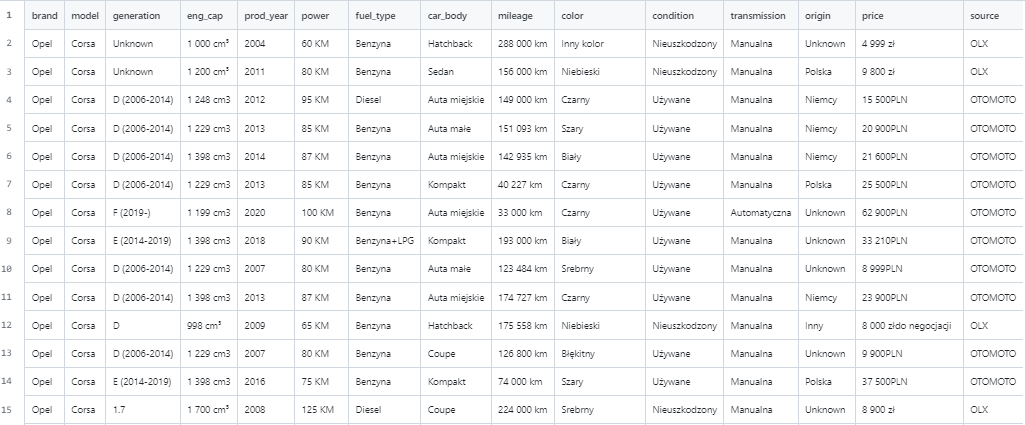
\includegraphics[width=\textwidth]{images/reprezentacyjny_zbior_danych_OLX_OTOMOTO.png}
    \caption{Reprezentacyjny zbiór danych z OTOMOTO i OLX, pokazujący częste wartości puste dla danych z OLX}
  \end{minipage}\hfill
  \begin{minipage}{0.45\textwidth}
    \centering
    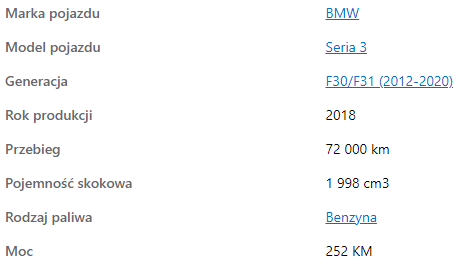
\includegraphics[width=\textwidth]{images/wycinek_danych_otomoto.png}
    \caption{Dane obligatoryjne na OTOMOTO}
  \end{minipage}\hfill
  \begin{minipage}{0.45\textwidth}
    \centering
    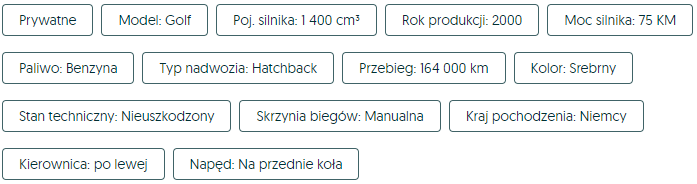
\includegraphics[width=\textwidth]{images/wycinek_danych_olx.png}
    \caption{Dane opcjonalne na OLX}
  \end{minipage}
\end{figure}

\subsection{Oczyszczanie danych}
Przed właściwą analizą danych, wymagają one wstępnego przetworzenia i oczyszczenia.

\begin{figure}[H]
    \centering
    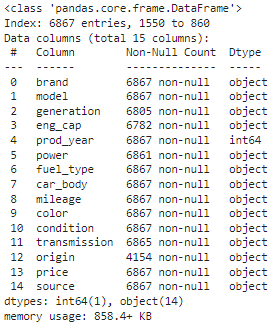
\includegraphics[width=0.5\textwidth]{images/typy_danych_w_dataframe.png}
    \caption{Typy danych do analizy}
\end{figure}

\begin{figure}[H]
    \centering
    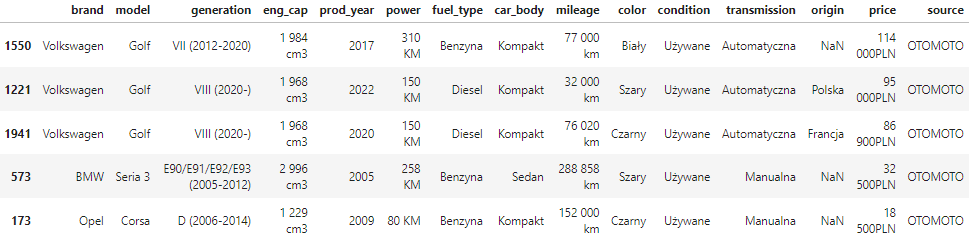
\includegraphics[width=1\linewidth]{images/reprezentacyjne_wartosci_z_jednostkami.png}
    \caption{Reprezentacyjny zbiór danych z nieusuniętymi jednostkami}
\end{figure}

Jak widać na powyższych spisach - jedynie rok produkcji jest od samego początku zapisany jako poprawny typ danych. Aby sprowadzić resztę danych do właściwej formy należy na tym etapie dla wszystkich wartości liczbowych usunąć jednostkę, by móc następnie rzutować wartości na typy liczbowe.

Dodatkowo dla ceny należy zamienić wartości podane w walutach zagranicznych na PLN (wykorzystana zostanie do tego biblioteka forex-python \cite{forex_python})

\begin{figure}[H]
    \centering
    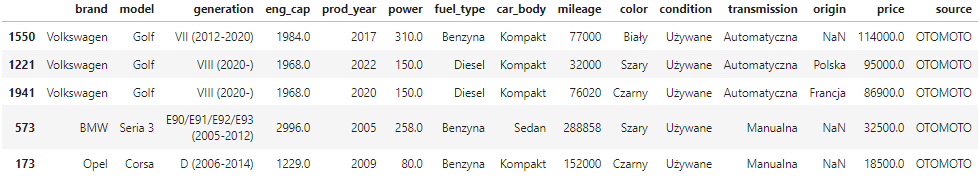
\includegraphics[width=1\linewidth]{images/reprezentacyjny_wycinek_danych_bez_jednostek.png}
    \caption{Reprezentacyjny wycinek danych po rzutowaniu typów}
\end{figure}

\section{Analiza i dalsze przetwarzanie przygotowanych danych}

\subsection{Eksploracyjna analiza danych}
Do celów wstępnej analizy wizualnej danych zostało wykorzystane narzędzie ProfileReport z modułu pythona: \href{https://pypi.org/project/ydata-profiling/}{ydata\_profiling}.

\subsection{Funkcja do analizy wartości odstających (outlierów)}\label{subsec:outlier_func}
Zanim poszczególne zmienne zostaną dogłębniej przeanalizowane, warto przygotować funkcję, która pomoże nam odfiltrować nadzwyczajnie, odstającą od reszty część danych - zwaną \textit{outlierami}. Zwykle nie chcemy analizować takich danych, gdyż w większości przypadków są to informacje nieprawdziwe, powstałe na skutek różnego rodzaju błędów i mogłyby one negatywnie wpływać na wyniki naszego modelu.
 
Utworzona funkcja klasyfikuje wartości jako odstające na podstawie ich \textbf{zscore} - jest to współczynnik oznaczający o ile odchyleń standardowych dana wartość różni się od oczekiwanej. Jeżeli wartość bezwzględna z \textbf{zscore} będzie większa od przyjętego progu, wówczas próbka zostanie sklasyfikowana jako odstająca. Za nasz próg przyjmiemy liczbę 3 - gdyż zgodnie z \textit{regułą trzech sigm} \cite{three_sigma_rule}: dla danych o rozkładzie normalnym, 99,7\% próbek, będzie mieścić się w granicach trzech odchyleń standardowych, po obu stronach wartości oczekiwanej.

\begin{figure}[H]
    \centering
    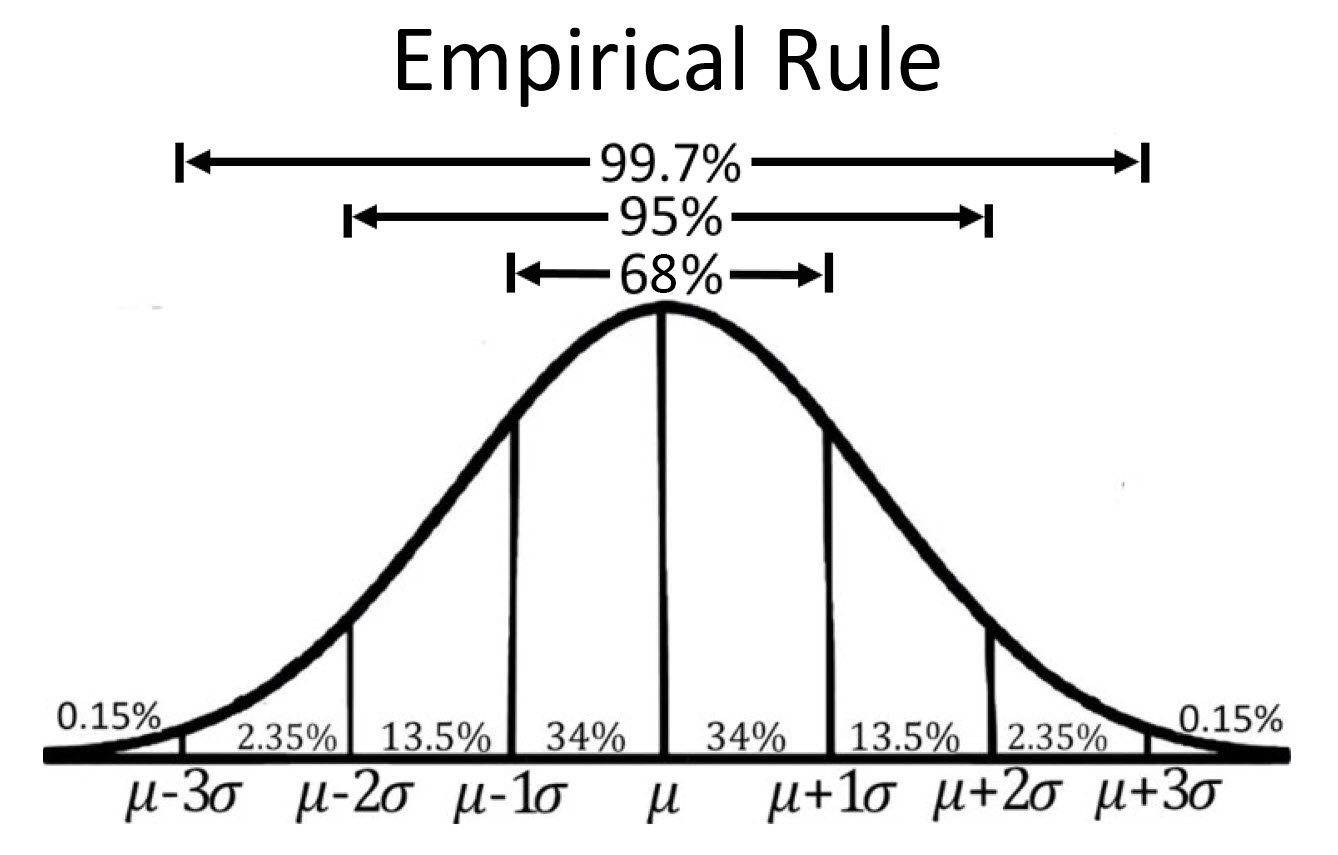
\includegraphics[width=0.75\linewidth]{images/regula_trzech_sigm.jpg}
    \caption{Reguła trzech sigm}
    \label{plt:three_sigm_rule}
\end{figure}

\subsection{Usuwanie duplikatów}
Pomimo, że teoretycznie na stronie internetowej, z ofertami samochodowymi nie powinno być żadnych powtórek, to jednak należy wziąć pod uwagę, że pobranie tak dużej ilości danych zajmuje trochę czasu (ponad 4 godziny dla prawie 7000 samochodów) i przez ten czas niektóre oferty mogą zostać dodane, usunięte lub odświeżone i pomimo ich pobrania, mogą one pojawić się znowu na następnych kartach. Dlatego też warto na tym etapie pozbyć się spowodowanych w ten sposób powtórzeń.

\subsection{Źródło}
Zmienna decyzyjna źródło, jest artefaktem pozostałym, po wersji scrapera, który pobierał dane również z OLX. Teraz, kiedy źródłem danych pozostało OTOMOTO, w tym polu występuje tylko jedna możliwa wartość. Można je więc od razu usunąć z naszych rozważań.

\subsection{Marka, model}
Zmienne decyzyjne marka, model oraz generacja, wspólnie tworzą 3-elementową krotkę, jednoznacznie wyróżniającą dany rodzaj samochodu na tle innych (np. Volkswagen Golf V). Jednak warto zwrócić uwagę, że (w przypadku wybranych do analizy pojazdów), sama generacja będzie wystarczająca do jednoznacznej identyfikacji typu pojazdu - gdyż konkretna generacja ma unikatową nazwę w obrębie danego modelu, który to przynależy pod daną markę - i nazwa tej generacji nie powtarza się dla żadnego innego modelu, jakiejkolwiek innej marki. Dzięki takiej zależności możemy zmniejszyć złożoność naszych danych i usunąc z nich obie te zmienne, zostawiając tylko generację. 

\subsection{Generacja}
\begin{figure}[H]
    \centering
    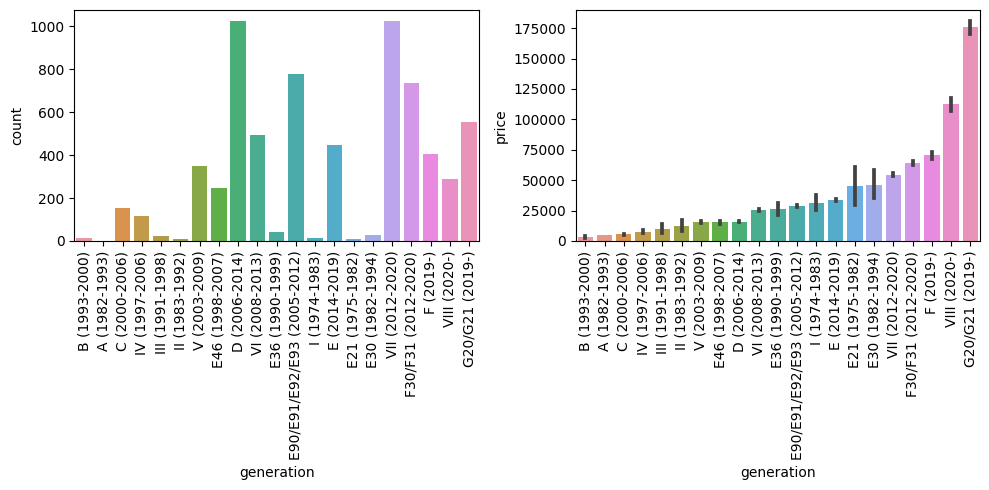
\includegraphics[width=1\linewidth]{images/generacja.png}
    \label{plt:generation}
    \caption{Histogram generacji oraz wykres zależności ceny od generacji}
\end{figure}

Jak można zauważyć z powyższych wykresów, występuje widoczna zależność pomiędzy generacją samochodu a jego ceną. Histogram również nie daje nam powodów do usunięcia tej zmiennej decyzyjnej z analizy. Poza tym, usuwając ją, stracilibyśmy możliwość sprawdzenia ceny samochodu, dla konkretnego typu pojazdu (jako zmienne losowe, zostałyby tylko parametry auta), a przecież takie było założenie naszego projektu - by estymować cenę \textbf{konkretnego auta} na podstawie jego parametrów technicznych - zatem generacja samochodu zdecydowanie musi pozostać w zbiorze analizowanych danych. 

\subsection{Pojemność silnika}
\begin{figure}[H]
    \centering
    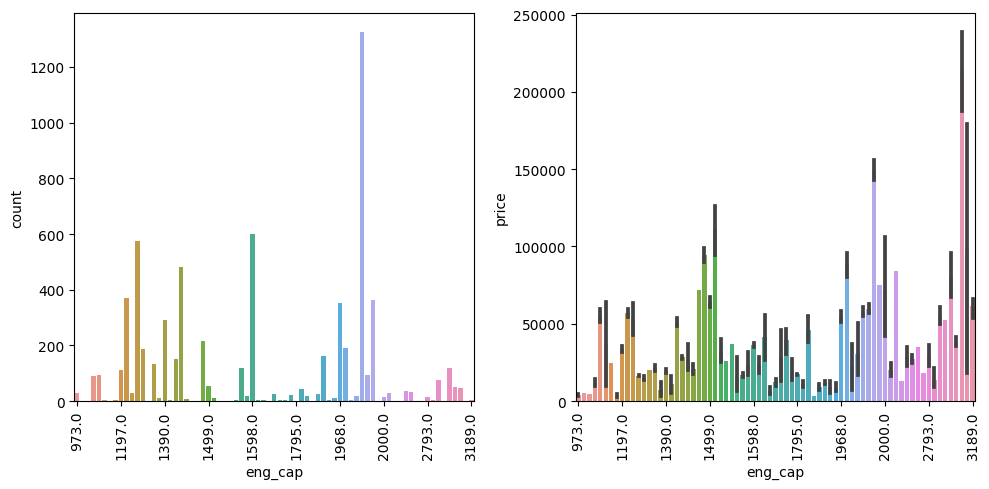
\includegraphics[width=1\linewidth]{images/pojemnosc_silnika.png}
    \label{plt:eng_cap}
    \caption{Histogram pojemności silnika oraz wykres zależności ceny od pojemności silnika}
\end{figure}

Jak widać na wykresie, nie mamy tutaj do czynienia z silną korelacją pomiędzy ceną a pojemnością silnika. Wykres rzeczywiście ma tendencję wzrostową, jednakże jest ona zaszumiona i mocno się waha. Z tego względu, po utworzeniu modelu zrobiłem eksperyment, w którym testowałem wpływ usunięcia pojemności silnika ze zbioru danych na metryki modeli. Okazało się, że wyniki były nieco lepsze przy pozostawieniu tej części danych - więc tak uczynię.

\subsection{Rok produkcji}
\begin{figure}[H]
    \centering
    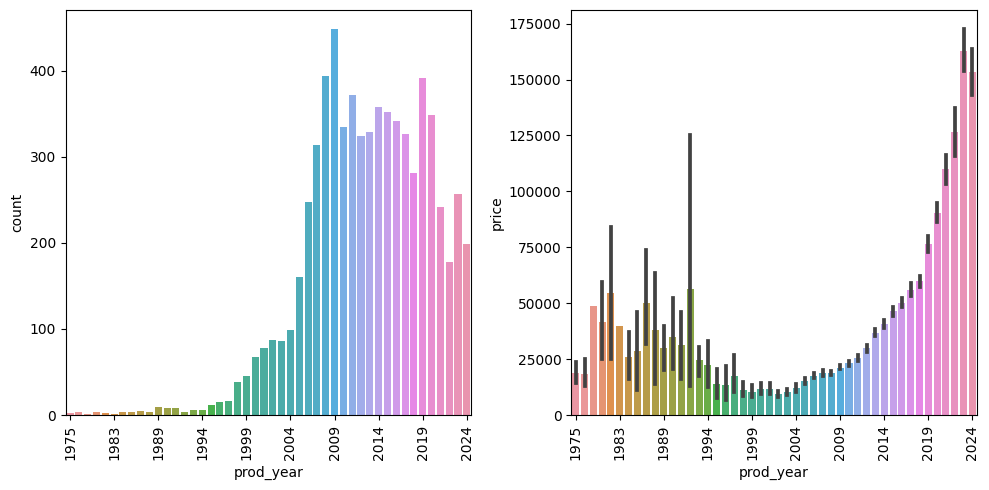
\includegraphics[width=1\linewidth]{images/rok_produkcji_przed.png}
    \label{plt:prod_year_bef}
    \caption{Histogram lat produkcji i wykres zależności ceny od roku produkcji}
\end{figure}

Jak można odczytać z wykresu, rok produkcji jest silnie skorelowany z ceną. Wyłania nam się ciekawa, paraboliczna zależność - najnowsze samochody są najdroższe, im auto jest starsze, tym cena jest niższa, ale do czasu. W pewnym momencie (około 2000 roku) wykres odbija w drugą stronę - samochody z ubiegłego wieku są uznawane za klasyki przez co ich cena (wraz z wiekiem) zaczyna rosnąć.

Z histogramu możemy zobaczyć, że wykres rozpoczyna się od 1975 roku, pomimo bardzo małej ilości samochodów aż do 1990 roku. Z tego względu warto odfiltrować dane pod kątem wartości odstających. Użyjemy do tego celu wcześniej wprowadzonej funkcji \ref{subsec:outlier_func}.
\begin{figure}[H]
    \centering
    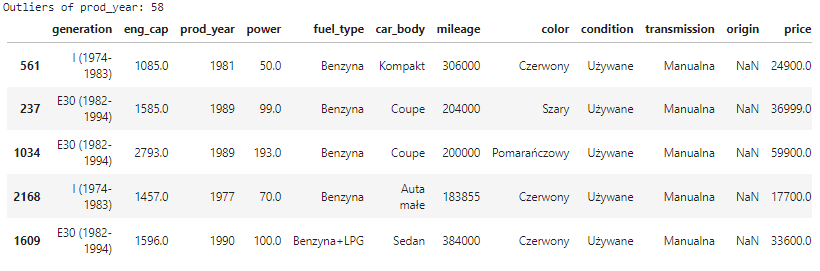
\includegraphics[width=0.9\linewidth]{images/reprezentacyjne_wartosci_odstajace_roku_produkcji.png}
    \caption{Reprezentacyjne wartości odstające roku produkcji}
\end{figure}

\begin{figure}[H]
    \centering
    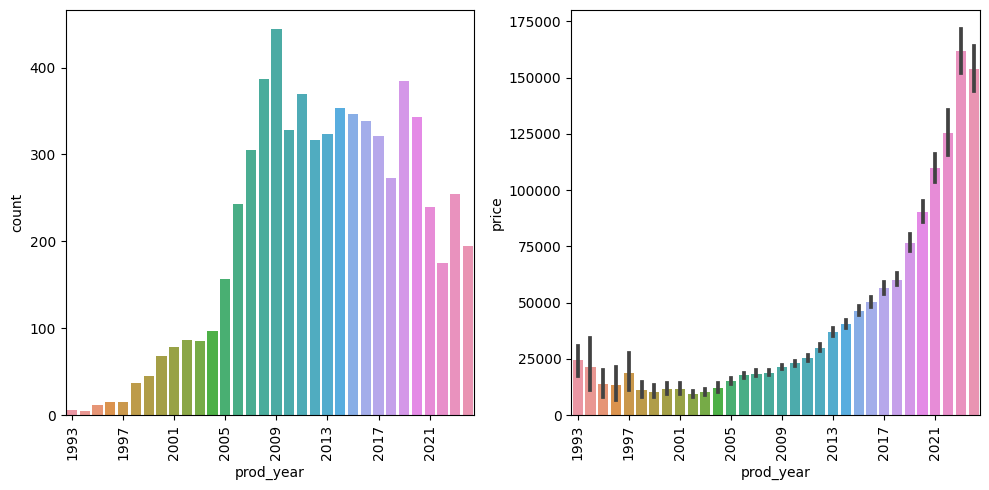
\includegraphics[width=1\linewidth]{images/rok_produkcji_po.png}
    \caption{Histogram lat produkcji i wykres zależności ceny od roku produkcji po odfiltrowaniu wartości odstających}
    \label{plt:prod_year_aft}
\end{figure}

Jak widać na nowym wykresie, nasza parabola przyjęła bardziej gładki kształt, a rozłożenie wartości na histogramie bardziej przypomina rozkład normalny niż wcześniej. 

\subsection{Moc}
\begin{figure}[H]
    \centering
    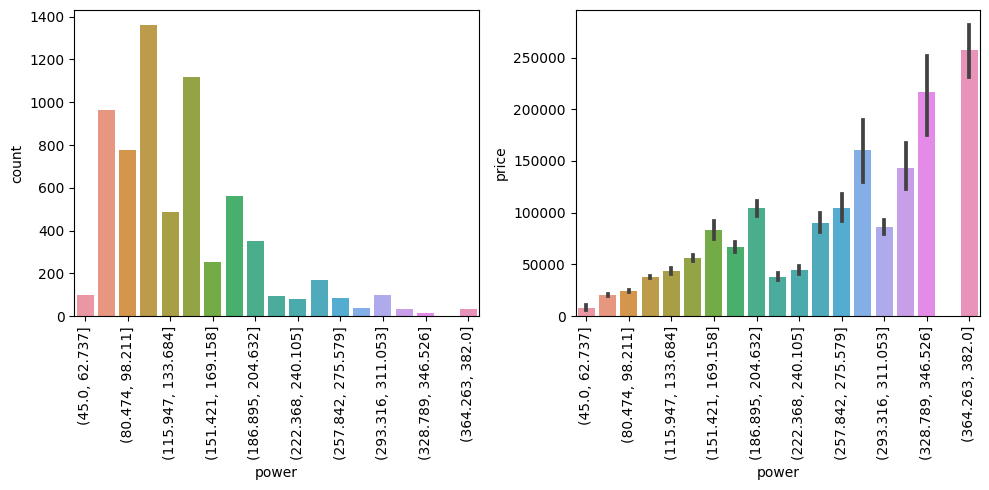
\includegraphics[width=1\linewidth]{images/moc_przed.png}
    \caption{Histogram mocy i wykres zależności ceny od mocy}
    \label{plt:power_bef}
\end{figure}
Wykres przedstawia całkiem gładką, wzrostową charakterystykę mocy w stosunku do ceny samochodu. Po odfiltrowaniu danych pod kątem ewentualnych wartości odstających - moc zostanie wykorzystana przy późniejszym uczeniu modelu.

%\newpage %TODO
\subsection{Rodzaj paliwa}
\begin{figure}[H]
    \centering
    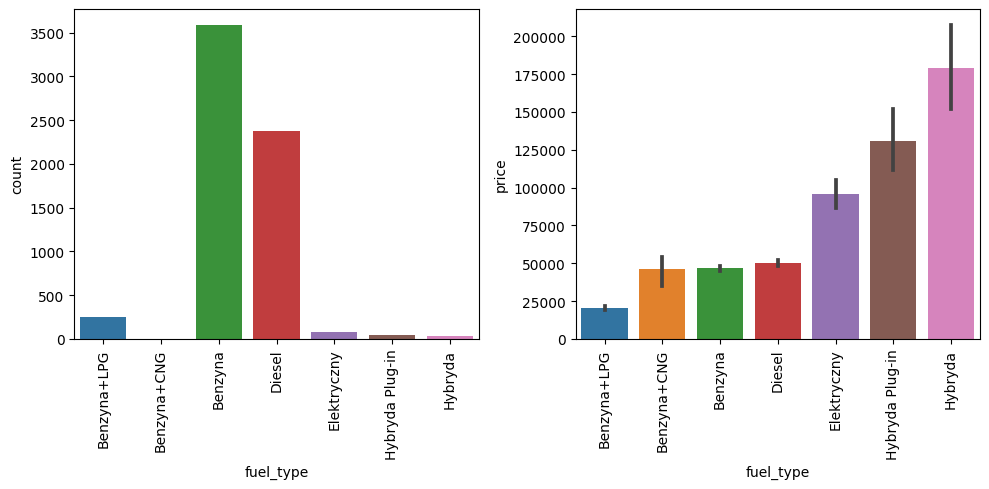
\includegraphics[width=1\linewidth]{images/typ_paliwa.png}
    \caption{Histogram rodzaju paliwa i wykres zależności ceny od rodzaju paliwa}
    \label{plt:fuel_type}
\end{figure}
Jak widać na histogramie - oprócz samochodów z silnikiem diesla i benzynowym, nie mamy zbyt wiele danych na temat innych rodzajów paliwa - z tego względu, pomimo zróżnicowania poziomu cen w zależności od użytego paliwa, nie będziemy rozważać tych danych w przypadku naszego modelu - dane są zbyt nierównomiernie rozłożone. 

\subsection{Typ nadwozia}
\begin{figure}[H]
    \centering
    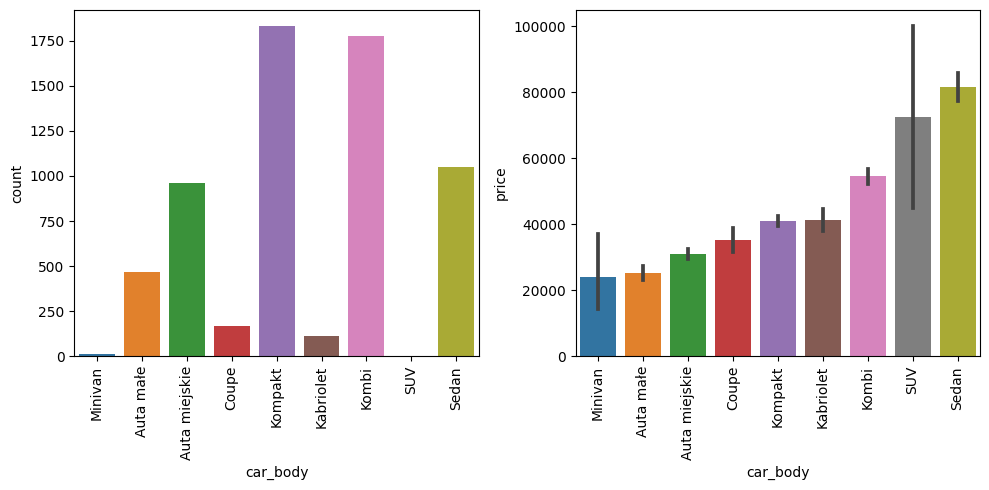
\includegraphics[width=1\linewidth]{images/rodzaj_nadwozia.png}
    \caption{Histogram typu nadwozia oraz wykres zależności ceny od nadwozia samochodu}
    \label{plt:car_body}
\end{figure}
Pomimo, że widać znaczące różnice w cenie dla samochodów z różnymi typami nadwozia, podobnie jak z rodzajami paliwa, nie mamy zbyt wiele próbek danych dla części z tych typów.

%\begin{figure}[H]
    %\centering
    %\includegraphics[width=0.25\linewidth]%{images/car_body_count_unique.png}
    %\caption{Zestawienie samochodów z %podziałem na różne typy nadwozi}
%\end{figure}


\begin{table}[H]
    \centering
    \begin{tabular}{crr}
       \textbf{Typ nadwozia} & \textbf{Liczba} & \textbf{\% wszystkich} \\ \hline
        Kompakt & 1829 & 28.681198 \\
        Kombi & 1777 & 27.865768 \\
        Sedan & 1050 & 16.465423 \\
        Auta miejskie & 961 & 15.069782 \\
        Auta małe & 465 & 7.291830 \\
        Coupe & 167 & 2.618786 \\
        Kabriolet & 115 & 1.803356 \\
        Minivan & 11 & 0.172495 \\
        SUV & 2 & 0.031363 \\
    \end{tabular}
    \caption{Zestawienie samochodów z podziałem na różne typy nadwozi}
\end{table}

Jak widać w powyższej tabeli, SUV'y i minivany nie stanowią nawet 1\% wszystkich danych i tylko 4 ze wszystkich rodzajów nadwozi przekraczają 10\% udziału wśród danych. Ze względu na takie zróżnicowanie, nie będziemy rozważać dalej tej zmiennej decyzyjnej.

%\newpage %TODO
\subsection{Przebieg}
\begin{figure}[H]
    \centering
    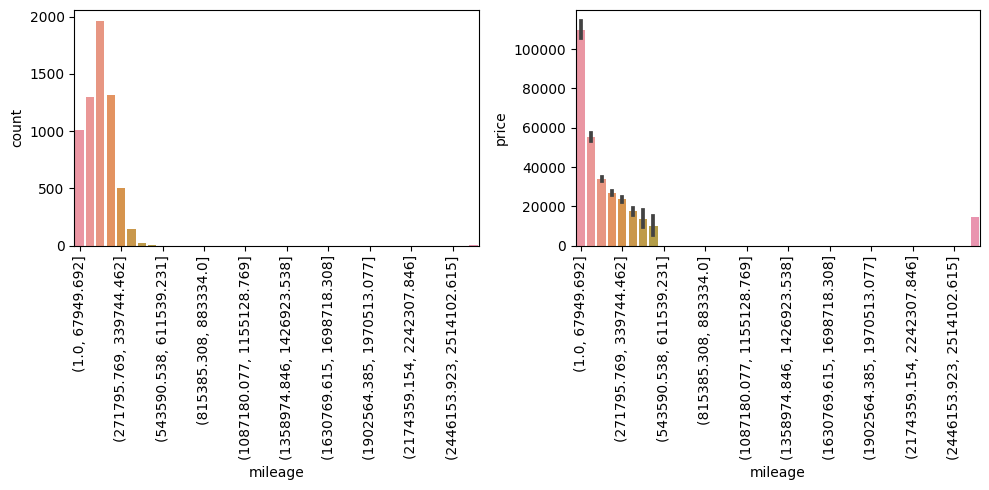
\includegraphics[width=1\linewidth]{images/przebieg_przed.png}
    \caption{Histogram przebiegu oraz wykres zależności ceny od przebiegu samochodu}
    \label{plt:mileage_bef}
\end{figure}

Jak widać na obu diagramach, większość danych umiejscowiona jest w przedziale do około 400 000km. Poza tym przedziałem na wykresie widać tylko jeden słupek na wartości ponad 2 500 000km. Nie widzę potrzeby brania pod uwagę całego tego przedziału tylko dla pojedynczych dodatkowych wartości, zatem przefiltruję je pod kątem wartości odstających.

\begin{figure}[H]
    \centering
    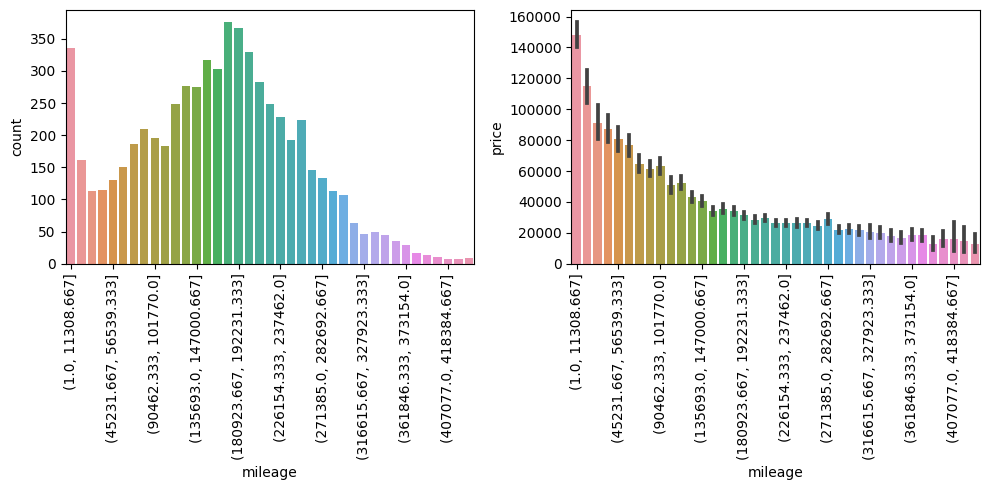
\includegraphics[width=1\linewidth]{images/przebieg_po.png}
    \caption{Histogram przebiegu oraz wykres zależności ceny od przebiegu samochodu po usunięciu wartości odstających}
    \label{fig:enter-label}
\end{figure}

Teraz histogram przebiegu bardzo przypomina rozkład Gaussowski. Zależność ceny od przebiegu również się wyklarowała. Korelacja okazała się być bardzo silna, a przebieg wykresu jest gładki i ma charakter spadkowy.
Zmienna decyzyjna w takiej postaci oczywiście zostaje do późniejszych zastosowań dla modeli.

%\newpage %TODO
\subsection{Kolor}
\begin{figure}[H]
    \centering
    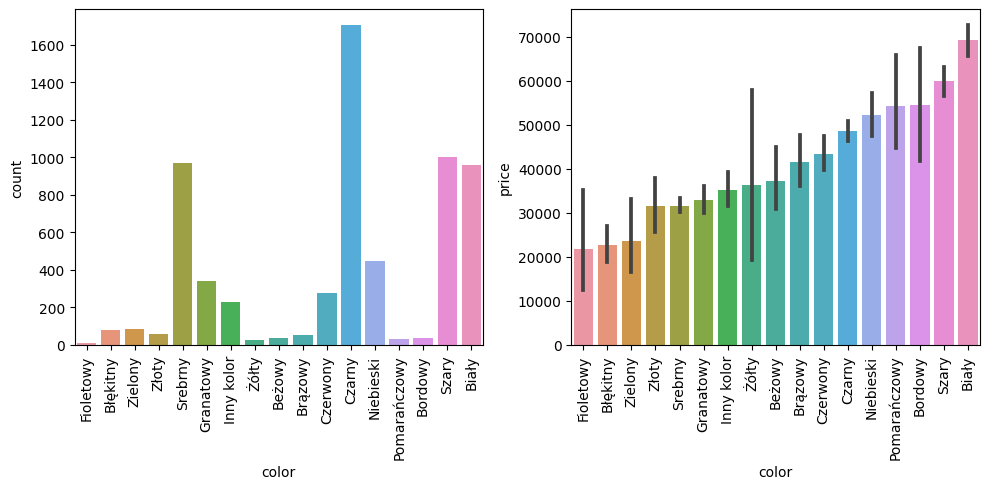
\includegraphics[width=1\linewidth]{images/kolor.png}
    \caption{Histogram koloru oraz wykres zależności ceny od koloru samochodu}
    \label{plt:color}
\end{figure}
Dla wielu kolorów samochodów, mamy bardzo mało danych. Tylko cztery spośród siedemnastu kolorów stanowią większość wśród danych. Pomimo więc wyraźnego zróżnicowania poziomu cen dla samochodów o różnych kolorach, zdecydowałem się odrzucić tę porcję danych z analizy.

%\newpage %TODO
\subsection{Stan}
\begin{figure}[H]
    \centering
    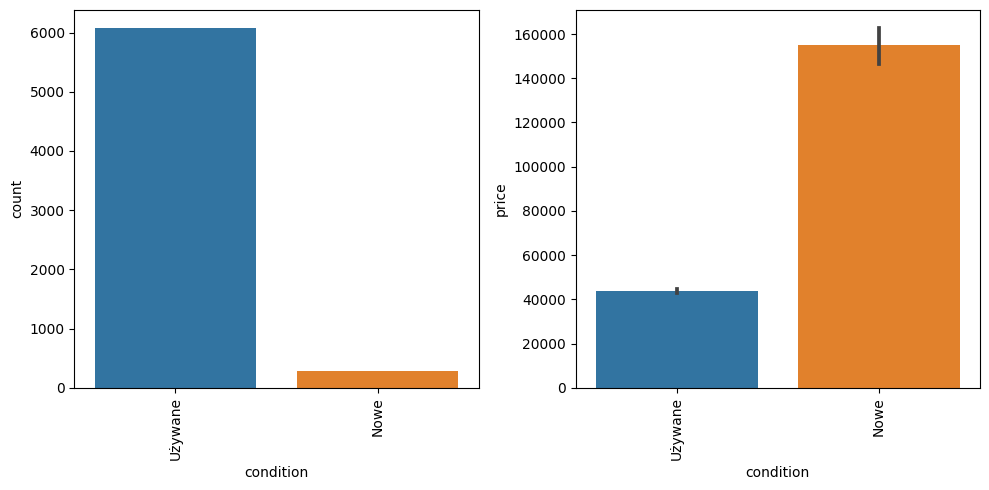
\includegraphics[width=1\linewidth]{images/stan.png}
    \caption{Histogram stanu oraz wykres zależności ceny od stanu samochodu}
    \label{plt:condition}
\end{figure}
Mamy do czynienia z silną przewagą w ilości samochodów używanych nad nowymi. Nie możemy jednak z tego powodu po prostu usunąć informacji o stanie, gdyż z drugiej strony nowe samochody są zauważalnie dużo droższe od używanych. Ze względu na tę silną korelację - pozostawimy te dane.

%\newpage %TODO
\subsection{Skrzynia biegów}
\begin{figure}[H]
    \centering
    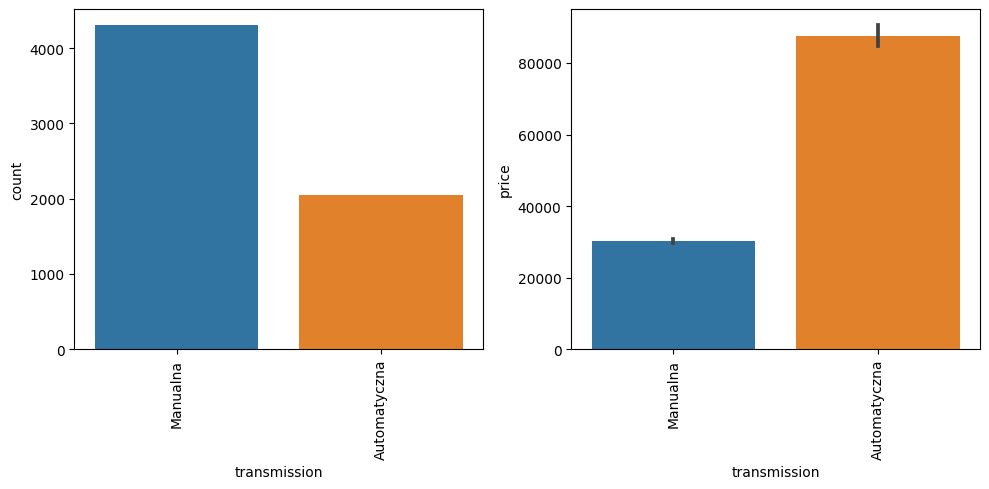
\includegraphics[width=1\linewidth]{images/skrzynia_biegow.png}
    \caption{Histogram rodzajów skrzyni biegów oraz wykres zależności ceny od rodzaju skrzyni biegów}
    \label{plt:transmission}
\end{figure}
W tym przypadku mamy ponad dwukrotną przewagę w ilości samochodów z manualną skrzynią biegów w stosunku do samochodów z automatyczną skrzynią. Skrzynia automatyczna natomiast jest średnio trzykrotnie droższa od manualnej. Warto zatem zostawić te dane do nauki dla przyszłych modeli.

%\newpage %TODO
\subsection{Pochodzenie}
\begin{figure}[H]
    \centering
    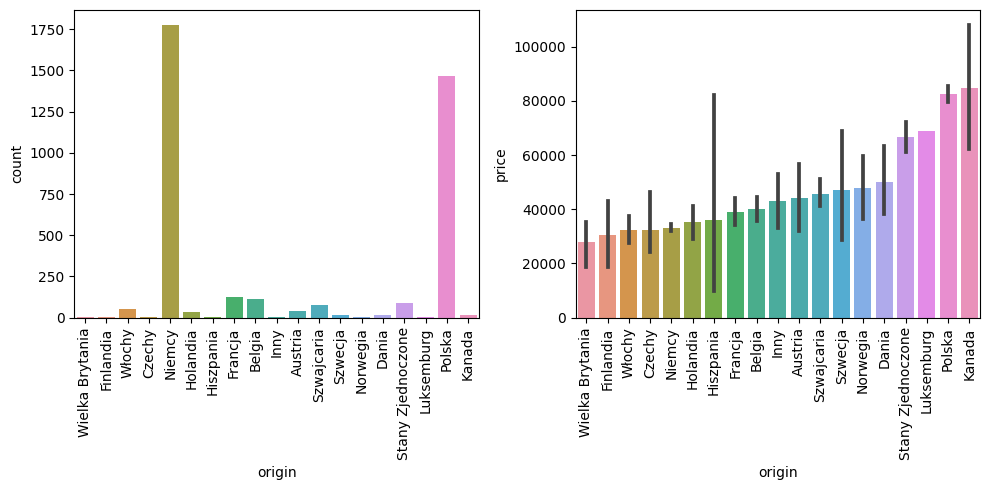
\includegraphics[width=1\linewidth]{images/kraj_pochodzenia.png}
    \caption{Histogram kraju pochodzenia oraz wykres zależności ceny od kraju pochodzenia samochodu}
    \label{plt:origin}
\end{figure}
Prawie wszystkie samochody pochodzą z Polski lub Niemiec. Mamy niestety zbyt wiele różnych innych krajów z przypisaną do siebie małą ilością samochodów, przez co nie powinniśmy ufać zależnością przedstawionym na wykresie. Dodatkowo, tylko przy nieco ponad 4000 samochodów, mamy niepusty kraj pochodzenia, czyli w przypadku niecałych 40\% przypadków kraj pochodzenia samochodu jest nieznany. Z obu tych względów rozsądnie będzie odrzucić tę porcję danych z dalszej analizy.

%\newpage %TODO
\section{Końcowe przetwarzanie danych}
\subsection{Uzupełnienie wartości pustych}
Do uzupełniania wartości pustych przyjęte zostały dwie strategie: po jednej dla danych ciągłych i kategorycznych.
\begin{itemize}
    \item \underline{Dane ciągłe:}

    tutaj strategia jest bardzo prosta - wszystkie dane są uzupełniane wartością średnią.

    \item \underline{Dane kategoryczne:}
    
    strategia jest następująca - dla każdej kategorii liczone jest prawdopodobieństwo jej wystąpienia i dla każdych uzupełnianych danych losowana jest kategoria zgodnie z policzonym wcześniej prawdopodobieństwem.
    
\end{itemize}

Po uzupełnieniu danych, należy sprawdzić, czy nie ma żadnych duplikatów, które mogły powstać przy usuwaniu zmiennych decyzyjnych lub przy wypełnianiu pól pustych i ewentualnie takie powtórzenia usunąć.

Na tym etapie, po przeprowadzonej analizie, jako że dane są już prawie gotowe jako wejście dla modeli, przedstawię macierz korelacji dla przetworzonych danych. Celem łatwej interpretacji, na macierzy zostaną tylko wartości numeryczne (bez zmiennych kategorycznych):

\begin{figure}[H]
    \centering
    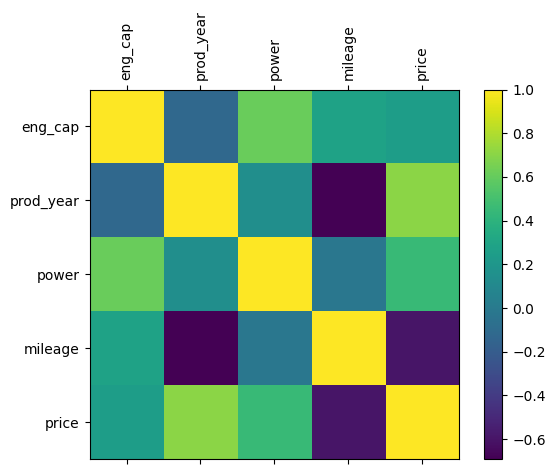
\includegraphics[width=0.75\linewidth]{images/macierz_korelacji.png}
    \caption{Macierz korelacji zmiennych numerycznych}
\end{figure}

Jak widać na przedstawionej macierzy, pojemność silnika oraz moc są całkiem dobrze skorelowane z ceną, ale to z rokiem produkcji cena ma najwyższy współczynnik korelacji - co z resztą było widać na poprzednich wykresach - które były najmniej zaszumione i najgładsze właśnie dla roku produkcji. Pozostała reszta - czyli przebieg samochodu wykazał bardzo wysoki ujemny współczynnik korelacji - co również ma odzwierciedlenie w kształcie poprzednich wykresów, które dla przebiegu były również jednymi z najgładszych i najbardziej równomiernie rozłożonych - tyle że w przeciwieństwie do wcześniej wymieonionych - wykres przebiegu miał charakter spadkowy - stąd ujemna wartość współczynnika.

\subsection{Kodowanie danych kategorycznych}
Wszystkie dane kategoryczne muszą zostać odpowiednio zakodowane celem odpowiedniej ich interpretacji przez model. Na rzecz tego projektu, przetestowałem dwa sposoby kodowania: \textit{one-hot} encoding oraz \textit{label encoding} \cite{encoding_types}. Pierwszy sposób dla jednej kolumny danych kategorycznych tworzy \textit{n} kolumn, gdzie \textit{n} jest liczbą wszystkich kategorii. Dla pojedynczej próbki tylko w jednej z tych kolumn może wystąpić wartość 1, w reszcie występuje 0 - stąd \textbf{one-hot}. Drugi sposób działa prościej - dla kolumny danych kategorycznych, przypisuje każdej kategorii liczbę (od 0 w górę) - zatem ilość kolumn się nie zmienia tylko zamiast kategorii jaka w tej kolumnie występowałą, zawarta jest od tej chwili odpowiadająca jej liczba.

Oba te sposoby kodowania dały bardzo podobne wyniki modeli, wybrałem więc label encoding - głównie dlatego, że niektórych kategorii było naprawdę dużo (np. generacji samochodu) - a mogłoby ich być jeszcze więcej dla nieco innych danych.

\begin{figure}[H]
    \centering
    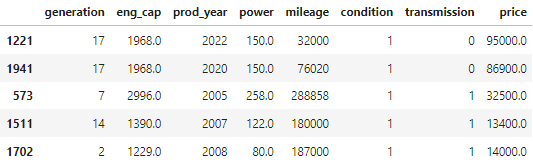
\includegraphics[width=1\linewidth]{images/reprezentacyjny_wycinek_danych_z_label_encoding.png}
    \caption{Reprezentacyjny wycinek danych po zastosowaniu label encodingu}
\end{figure}

\subsection{Podział danych}
Na tym etapie dane, przechowywane do tej pory w jednolitej formie, zostaną podzielone na dwa podzbiory: zbiór treningowy - dla nauki modelu, oraz zbiór testowy - do testowania modelu, w stosunku 3:1, gdyż po przeprowadzonych testach - taki właśnie stosunek dawał najlepsze rezultaty.

\subsection{Normalizacja}
Po zakodowaniu danych kategorycznych, należy znormalizować część zbioru danych, zawierającą zmienne decyzyjne - zarówno część testową jak i treningową. Polega to na przekształceniu każdej zmiennej losowej do zmiennej rozkładu normalnego o parametrach $\mu=0$ oraz $\sigma=1$. Wzorem, normalizacja przedstawia się następująco:
\begin{equation}
    \overline{X}=\frac{X-\mu}{\sigma}
\end{equation}
Operacja ta wykonywana jest po to, żeby wartości wszystkich zmiennych dezycyjnych zawierały się w podobnych przedziałach - aby żadna ze zmiennych nie wyhylała się wartościami ponad inne i żeby przez to model nie faworyzował jej wśród reszty \cite{normalization}.

Dlatego też normalizujemy tylko zmienne decyzyjne, a cena może pozostać nieznormalizowana, gdyż jest wyjściem modelu, a nie jego wejściem.

\section{Wybór modeli}
Proces obróbki danych został zakończony. Teraz nadszedł czas na wybór modeli, dla których dane te zostaną dopasowane. Na cel projektu rozważę następujące modele:
\begin{itemize}
    \item Random Forest
    \item Decision Tree
    \item Gradient Boosting
\end{itemize}

\subsection{Szukanie najlepszych parametrów modelu}
Każdy model przyjmuje inne parametry, decydujące o poziomie jego dopasowania do danych. 

Aby dobrać parametry, dające jak najlepsze wyniki, użyjemy tzw. Grid Search \cite{grid_search_cv}. Polega to na tym, że dla zadanej siatki parametrów (różnych wartości podanych dla konkretnych parametrów modelu), sprawdzane są wszystkie możliwe kombinacje. Dodatkowo Grid Search przjmuje charakterystyczny parametr $cv$ - cross-validation. Określa on na ile części zostaną podzielone podane dane, np. dla $cv=5$, dane zostaną podzielone na 5 części, gdzie stosunek treningowych do testowych wynosi 4:1. Model zostanie przetestowany dla każdego możliwego podziału na dane testowe i treningowe - w tym wypadku będzie 5 możliwości takiego podziału.

\subsection{Decision Tree}
Drzewo decyzyjne \cite{decision_tree} to jeden z podstawowych modeli uczenia maszynowego używanych do zadań klasyfikacji i regresji. Model ten działa poprzez rekurencyjne dzielenie danych na mniejsze podzbiory, tworząc strukturę drzewa, gdzie każdy węzeł odpowiada decyzji na podstawie wartości pewnej cechy.

Najważniejsze parametry drzewa decyzyjnego to:
\begin{itemize}
    \item criterion: Funkcja oceny podziału, np. “squared\_error”, “friedman\_mse”, “absolute\_error”, “poisson”
    \item splitter: Strategia użyta do wyboru podziału dla każdego węzła: “best” - najlepszy podział, “random” - najlepszy losowy podział
    \item max\_depth: Maksymalna głębokość drzewa. Ograniczenie głębokości drzewa zapobiega jego nadmiernemu dopasowaniu (overfitting).
    \item max\_features: Liczba cech rozważanych przy każdym podziale. Może być wartością absolutną, procentową lub "sqrt" (pierwiastek kwadratowy liczby cech) lub "log2".
    \item min\_samples\_split: Minimalna liczba próbek wymagana do podziału węzła. Większe wartości pomagają w uniknięciu nadmiernego dopasowania.
    \item min\_samples\_leaf: Minimalna liczba próbek, które muszą znajdować się w liściu. Wyższe wartości mogą poprawić ogólną stabilność modelu.
\end{itemize}

\subsection{Random Forest}
Las losowy \cite{random_forest} to złożony model uczenia maszynowego, który łączy wiele drzew decyzyjnych, aby poprawić dokładność i kontrolować nadmierne dopasowanie. Każde drzewo w lesie losowym jest trenowane na losowym podzbiore danych z użyciem losowych podzbiorów cech, co zwiększa różnorodność i ogólną wydajność modelu.

Najważniejsze parametry lasu losowego to:
\begin{itemize}
    \item n\_estimators: Liczba drzew w lesie. Większa liczba drzew zwykle poprawia dokładność modelu, ale zwiększa również czas obliczeń.
    \item max\_depth: Maksymalna głębokość drzew. Może być używana do kontrolowania złożoności każdego pojedynczego drzewa.
    \item max\_features: Podobnie jak w przypadku Decision Tree.
    \item min\_samples\_split i min\_samples\_leaf: Podobnie jak w drzewach decyzyjnych, parametry te pomagają kontrolować złożoność modeli i przeciwdziałać nadmiernemu dopasowaniu.
\end{itemize}

\subsection{Gradient Boosting}
Gradient Boosting \cite{gradient_boosting} to zaawansowana technika uczenia maszynowego, która iteracyjnie łączy słabe modele, takie jak małe drzewa decyzyjne, aby tworzyć silny model. Każde kolejne drzewo koryguje błędy popełnione przez poprzednie drzewa, co prowadzi do coraz lepszej wydajności modelu.

Najważniejsze parametry gradientowego boostingu to:

\begin{itemize}
    \item loss: Optymalizowana funkcja straty - model wykorzystuje tę funkcję, celem weryfikacji, czy w kolejnych iteracjach algorytmu, przewidywania modelu uległy poprawie. 
    \item n\_estimators: Liczba drzew w sekwencji. Większa liczba estymatorów może poprawić dokładność, ale zwiększa również ryzyko nadmiernego dopasowania.
    \item learning\_rate: Szybkość uczenia, która skaluje wkład każdego drzewa. Mniejsza wartość learning\_rate wymaga większej liczby estymatorów, aby osiągnąć ten sam poziom wydajności.
    \item max\_depth: Maksymalna głębokość każdego drzewa. Kontroluje złożoność każdego modelu bazowego.
    \item subsample: Proporcja próbek używana do trenowania każdego drzewa. Wartości poniżej 1.0 mogą pomóc w redukcji wariancji i nadmiernego dopasowania.
    \item min\_samples\_split i min\_samples\_leaf: Parametry te, podobnie jak w drzewach decyzyjnych i lasach losowych, kontrolują minimalną liczbę próbek wymaganą do podziału węzła i minimalną liczbę próbek w liściu.
\end{itemize}

\section{Dopasowywanie modelu}
Używając wybranych modeli wraz z siatkami parametrów, używamy wprowadzoną wcześniej metodę Grid Search w celu jak najlepszego dopasowania modeli do danych.

Dla poszczególnych modeli, parametry prezentują się następująco:
\begin{itemize}
    \item Decision Tree
    \begin{itemize}
        \item splitter: ['best', 'random'],    
        \item max\_depth: [None, 10, 20, 30], 
        \item min\_samples\_split: [2, 5, 10],
        \item min\_samples\_leaf: [1, 2, 4],
        \item max\_features: ['sqrt', 'log2']
    \end{itemize}
    
    \item Random Forest
    \begin{itemize}
        \item n\_estimators: [100, 200, 300],
        \item max\_depth: [None, 5, 10],
        \item min\_samples\_split: [2, 5, 10] 
    \end{itemize}

    \item Gradient Boosting
    \begin{itemize}
        \item loss: ['squared\_error', 'huber', 'quantile'],
        \item max\_depth: [3, 5],
        \item min\_samples\_split: [2, 5],
        \item min\_samples\_leaf: [1, 4]
    \end{itemize}

\end{itemize}

Dodatkowo każdy z modeli posiada parametr SEED - określający ziarno losowości - celem reprodukcji eksperymentów.

\subsection{Metryki}
Teraz czas przejść do metryk użytych aby opisać wyniki uzyskane przez modele.

\subsubsection{Mean absolut error}
Wzór:
\[
\text{MAE} = \frac{1}{n} \sum_{i=1}^{n} |\hat{y}_i - y_i|
\]
Jest to najbardziej podstawowa metryka, użyta do ocenienia modeli. Określa ona jak duży błąd jest popełniany przez model w predykowaniu ceny dla samochodu \cite{mean_absolute_error}.

\begin{table}[H]
    \centering
    \begin{tabular}{cc}
        \textbf{Model} & \textbf{Wynik} \\ \hline
        Decision Tree & 9878.346356 \\
        Random Forest & 7603.196992 \\
        Gradient Boosting & 7681.683557
    \end{tabular}
    \caption{MAE różnych modeli}
\end{table}

Można więc, dla przykładu, stwierdzić, że cena samochodu predykowana przez Random Forest, wynosi: $cena\_auta \pm 7603.20 PLN$

\subsubsection{Root mean squared error}
Wzór:
\[
\text{RMSE} = \sqrt{\frac{1}{n} \sum_{i=1}^{n} (\hat{y}_i - y_i)^2}
\]
Będzie to najważniejsza metryka naszych modeli - jej również używa Grid Search, więc to pod nią głównie model będzie dopasowany. Różni się ona od MAE m.in. tym, że jest wrażliwsza na wartości odstające - i jej wartość jest zawsze wyższa lub równa wartości MAE dla jednych danych. Z tego względu, aby oceniać nasz model też pod względem 'konsekwentnego' działania (czy nie robi pojedynczych, ale dużych błędów), użyjemy tej metryki \cite{root_mean_squared_error}.

\begin{table}[H]
    \centering
    \begin{tabular}{cc}
        \textbf{Model} & \textbf{Wynik} \\ \hline
        Decision Tree & 16654.488647 \\
        Random Forest & 12982.622761 \\
        Gradient Boosting & 13359.364812
    \end{tabular}
    \caption{RMSE różnych modeli}
\end{table}

\subsection{Metryka niestandardowa}
Ta metryka to właściwie procentowa wersja metryki RMSE, powstała po to, by klarownie przedstawić porównanie użytych modeli, za pomocą błędu względnego. Metryka ta, w przeciwieństwie do pozostałych, zwiększa swoją wartość (maksymalnie 1) wraz z polepszaniem się modelu. Jest ona liczona następująco:
\begin{equation}
    \text{METRYKA} = 1 - \frac{\sqrt{\frac{1}{n} \sum_{i=1}^{n} (\hat{y}_i - y_i)^2}}{\frac{1}{n} \sum_{i=1}^{n}y_i}
\end{equation}

\section{Wyniki}
Używając wprowadzonej wyżej funkcji, wyniki uzyskane przez modele prezentują się następująco:

\begin{table}[H]
    \centering
    \begin{tabular}{cc}
        \textbf{Model} & \textbf{Wynik} \\ \hline
        Decision Tree & 0.656413 \\
        Gradient Boosting & 0.724392 \\
        Random Forest & 0.732164
    \end{tabular}
    \caption{Końcowe metryki modeli}
    \label{tab:metrics_end_results}
\end{table}

\begin{figure}[H]
    \centering
    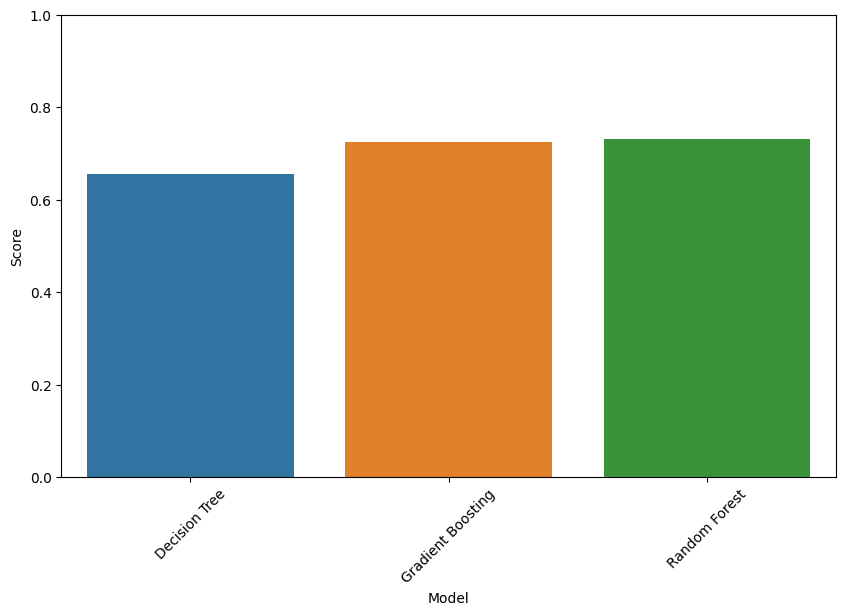
\includegraphics[width=1\linewidth]{images/metryki_modeli.png}
    \caption{Diagram końcowych metryk modeli}
    \label{plt:metrics}
\end{figure}

Dodatkowo, celem demonstracji jak najlepszy z modeli, tj. Random Forest radzi sobie na danych testowych, poniżej widnieje wykres przedstawiający wycinek danych testowych, przedstawionych jako połączone punkty, reprezentujące cenę (true) oraz drugi wykres, który przedstawia jak model te dane predykuje (predicted).

\begin{figure}[H]
    \centering
    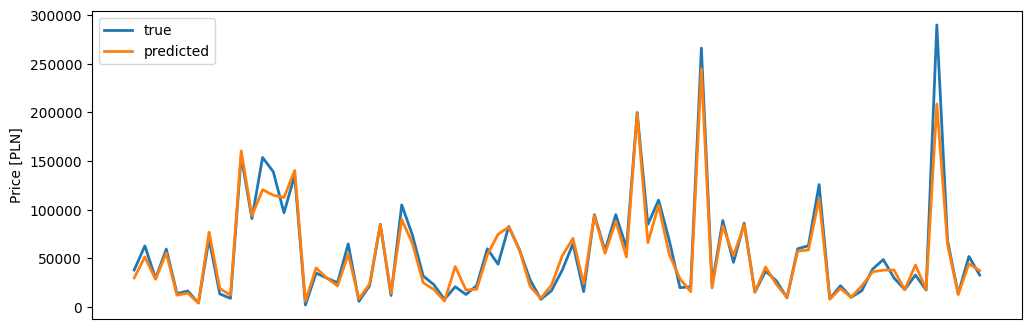
\includegraphics[width=1\linewidth]{images/najlepszy_model_predykcja.png}
    \caption{Wycinek danych testowych i ich predykcja przez model}
\end{figure}

\section{Wnioski}
Model \textbf{Random Forest} uzyskał najlepszy wynik, osiągając około 73,22\%. \textbf{Gradient Boosting} był niecały procent gorszy, natomiast \textbf{Decision Tree} aż 7,6\% gorszy. Wynika to z faktu, że zarówno Random Forest, jak i Gradient Boosting są metodami opartymi na drzewach decyzyjnych. Random Forest tworzy wiele drzew decyzyjnych i łączy ich wyniki, co zwiększa stabilność i dokładność modelu. Gradient Boosting natomiast tworzy sekwencję drzew, z których każde kolejne drzewo koryguje błędy poprzednich, co także poprawia wydajność. Z tego powodu oba te modele zazwyczaj przewyższają pojedyncze drzewo decyzyjne. Pomimo tych różnic, ich wspólna podstawa w drzewach decyzyjnych sprawia, że wyniki są do siebie stosunkowo zbliżone.

Modele całkiem dobrze poradziły sobie predykowaniem użytych danych, jednak ze względu na wielowymiarowość i nieliniowe zależności danych - metryka modeli nie była na bardzo wysokim poziomie. Uważam jednak, że jak na stopień skomplikowania analizowanych danych - rezultaty są akceptowalne.

Dodatkowo, wyniki projektu ukazują, że to przebieg oraz rok produkcji samochodu mają największe znaczenie w kształtowaniu się jego ceny i właśnie na te aspekty należy w dużym stopniu zwracać uwagę przy wyborze auta.

\newpage
\bibliographystyle{plain}
\bibliography{references}

\end{document}
